%Imperfection and time: modelling imperfect time (generally)


%Modelling imperfect time in temporal databases


%Guy's suggestion: instead of imprecision, use imperfection which is more general.
\subsubsection{Imperfection and time}
Representing imprecision and its semantics when dealing with time has been studied for a long time. Several proposals for representing and computing imprecise time indications can be found in \cite{DeCaluwe1997,DeTre1997}. Also, the changes between several granularities can be seen as a source of imprecision \cite{Devos1998}.

In the proposal section we will consider two kinds of imperfection:
\begin{itemize}
\item \textbf{Imperfection in the database} the knowledge about the temporal data contains some imperfection. E.g., a database record shows that \emph{`The car is in the garage around April.'}
 \item \textbf{Imprecision in the query specification} denotes the imprecision in the specification of temporal criteria by the user, when querying. E.g., \emph{`The user wants to obtain a car which is red and which is in the garage around April.'}
\end{itemize}

\subsubsection{Representation}
Several proposals for managing uncertain time in a database exist. Some proposals work with rough sets \cite{Qiang2009}, other proposals rely on possibility distributions for representing uncertainty in time \cite{Dyreson1998,Garrido2009,Galindo2001}. In order to compare temporal possibility distributions, extensions of the classical Allen's operators \cite{Allen1983} are defined in \cite{Ohlbach2004,Nagypal2003,Dubois2003a,Schockaert2008}.
%In the proposal section, we will follow the representation by means of possibility distributions, in order to work with both satisfaction and dissatisfaction degrees. Also, in order to work properly with fuzzy operators, the underlying domain should be numeric. 
% Take a look into this:
%In this paper, the representation for the dates will follow the Julian Day Number (JDN) representation \cite{Dir96}.

%If the starting points and/or the end points of the interval representing the time are not known precisely, it is easy to fuzzify them, using, e.g., two triangular possibility distributions.


In order to deal with uncertainty in time intervals, several proposals are made. Here, two approaches are introduced: the first one, based on \emph{Fuzzy Validity Period}~\cite{Garrido2009} and the second one based on \emph{Possibilistic Valid-time Period}~\cite{JoseEnriquePons2012}.

\begin{definition}
A \textbf{Fuzzy Validity Period} (\emph{FVP}) is defined as a fuzzy time interval specifying when the data regarding an object is valid. A fuzzy time interval is then the fuzzification of a crisp time interval.
\end{definition}
Several options to transform possibility distributions corresponding to the fuzzy starting point and the fuzzy end point into one consistent FVP exist \cite{Garrido2009}, e.g (Fig. \ref{fig:fuzzy-validity-period}):
\begin{itemize}
\item The \textbf{convex hull} approach is the most intuitive approach. The resulting FVP is the convex hull of the union of both fuzzy sets.
\item The \textbf{uncertainty preserving} approach is less intuitive but more realistic. The amount of uncertainty is maintained at the edges of the possibility distribution representing the FVP \cite{Garrido2009}.
\end{itemize}

%%%%%%
% FUZZY VALIDITY PERIOD
%%%%%%
\vspace*{13pt}
\begin{center}
{
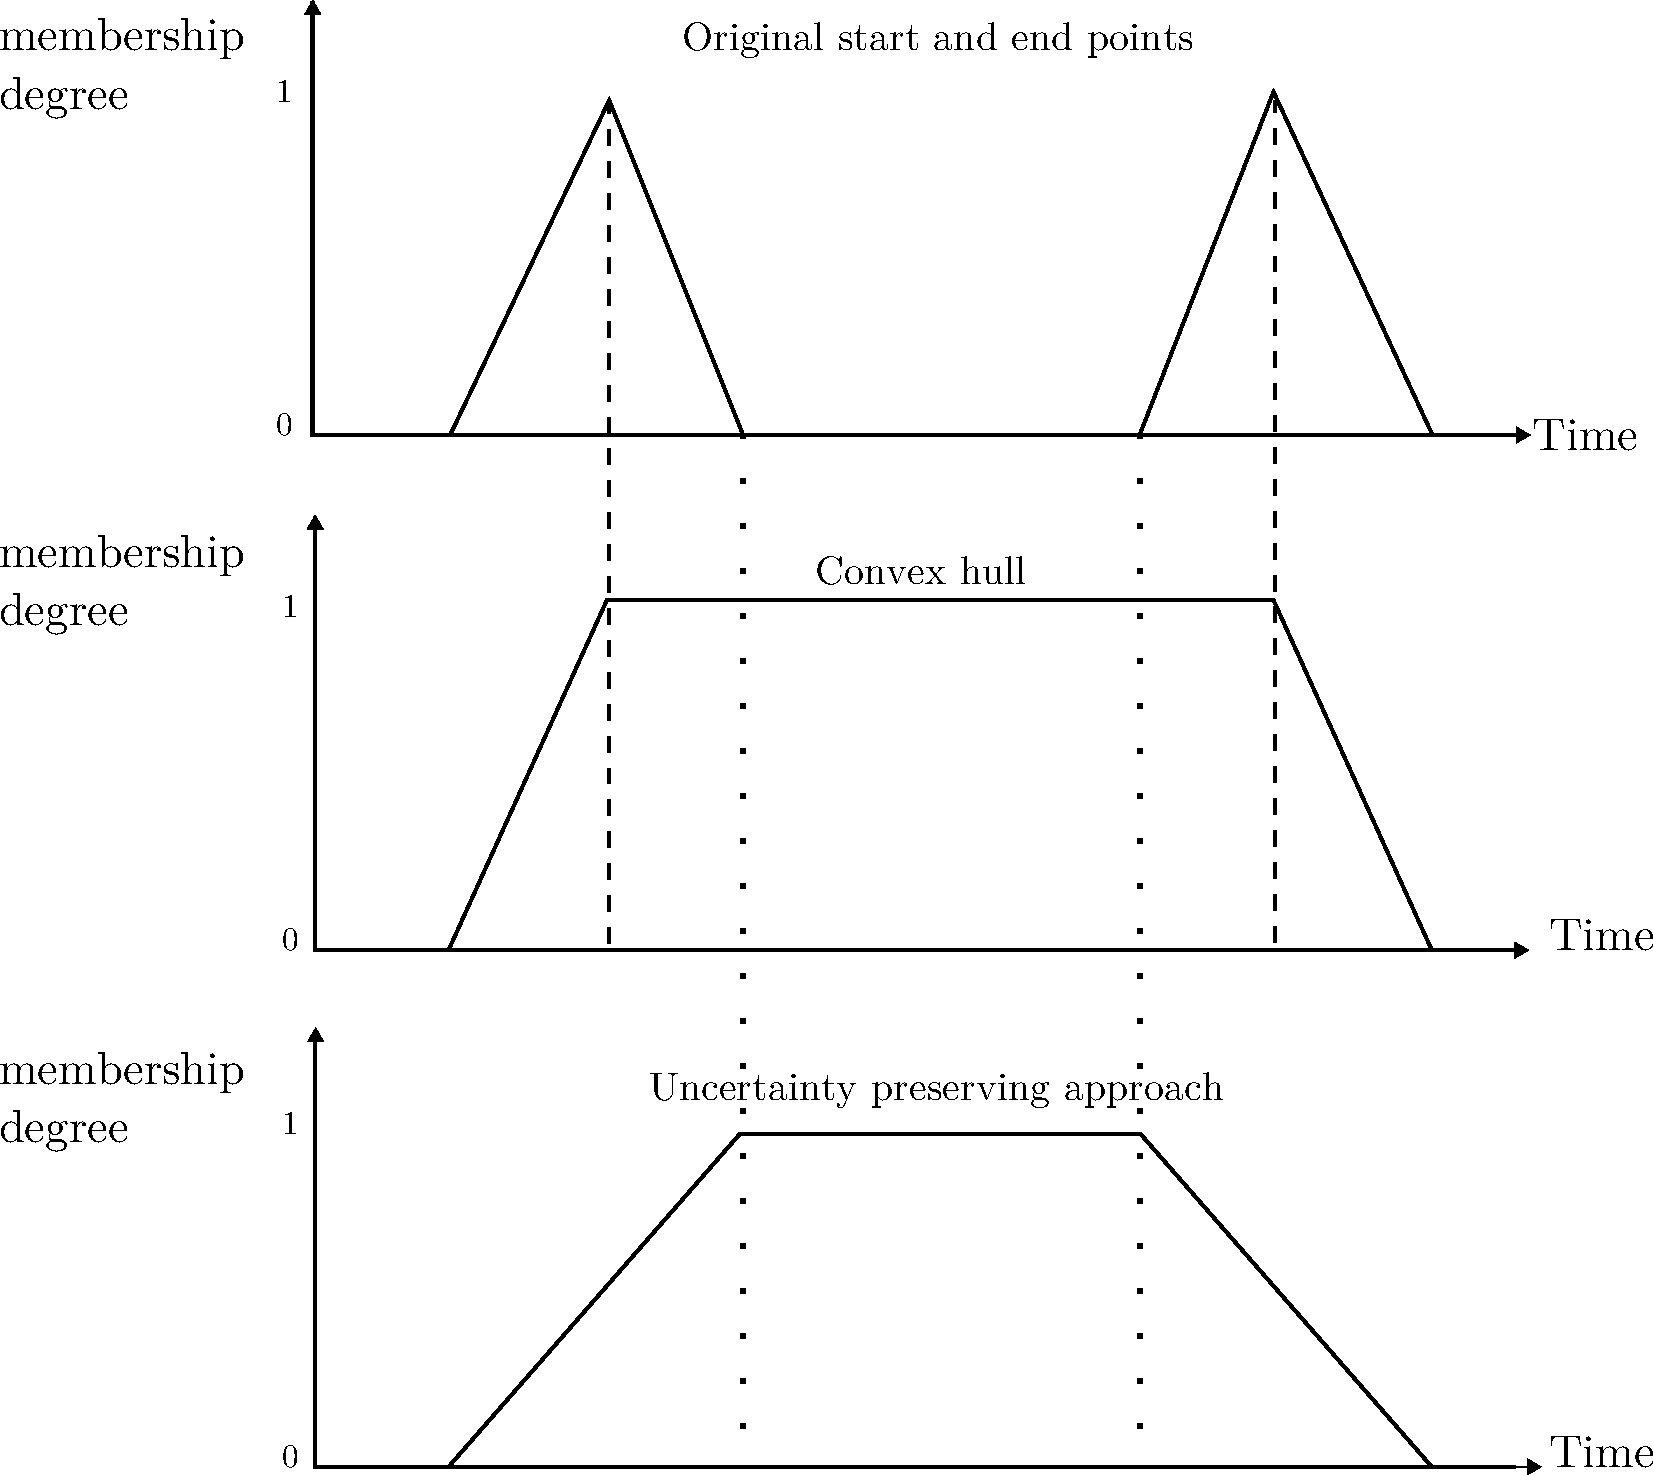
\includegraphics[scale=0.25]{./graphs/comparisoncv.pdf}

}
\end{center}
%\centerline{ 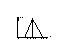
\psfig{file=./graphs/Y-time-point.eps}}
\vspace*{10pt}
\fcaption{\label{fig:fuzzy-validity-period}Transformation to obtain the FVP. The top graph shows the two triangular possibility distributions. The middle graph shows the convex hull validity period, the bottom one shows the result of the second transformation, which maintains the imprecision.}
%  \label{fig:fuzzy-validity-period}
\vspace*{13pt}

\begin{definition}
A \textbf{Possibilistic Valid-time Period} (\emph{PVP}) is an ill-known interval in time specifying when the data regarding an object is valid.
\end{definition}
A PVP is an ill-known interval in the sense of definition \ref{def;possibilistic-variable}, section \ref{subsec:possibilistic-variables}. Note that this representation is \emph{disjunctive}: the PVP represents only one crisp time interval, but that for some reason it is (partially) unknown.

The ill-known interval approach has many advantages from the representation by the FVP as demonstrated in \cite{Pons2011},\cite{Pons2012}. Table \ref{tbl:comparative-pvp-fvp} is a comparative between PVP and FVP. The following list defines the items in the comparative:

\begin{enumerate}
\item Domain: The domain of the possibility distribution modelled by the approach.
\item Implementation of relationships: How to implement a relationship.
\item Allen's relations: Are the Allen's relations defined?
\item Storage: The way the data is stored in the database.
\item Possibility measures: Does the framework provides always a possibility measure for any relation between the temporal elements?
\item Necessity measures:  Does the framework provides always a necessity measure for any relation between the temporal elements?
\end{enumerate}


%%
%% comparison table between pvp and fvp.
%%
\vglue13pt
%\begin{table}[htbp]
\tcap{Comparative PVP vs FVP}
%\centerline{\small DATA TYPES}
\vglue-6pt
\centerline{\small\baselineskip=13pt
\begin{tabular}{c p{2cm} p{2cm}}\\
Item & PVP & FVP\\
\hline
(1) & $\Pow(\R)$ & $\R$ \\
(2) & Ill-known constraints. & Ad-hoc operators. \\
(3) & $\checkmark$ & - \\
(4) & Two distributions one for each endpoint. & Only one distribution. \\ 
(5) & $\checkmark$ & $\checkmark$ \\
(6) & $\checkmark$ & - \\
\hline\\
\end{tabular}
\label{tbl:comparative-pvp-fvp}
} 

In the rest of the paper we will work only with PVP to represent valid-time intervals.
